\section{Environmental Impact}
The environmental impact of the plant is assessed based on the following indicators: GHG emissions intensity, water usage, and land use.

The assessment is conducted on the optimized operational scenario in which, for the first 20 years, both reactors are dedicated exclusively to electricity production and sale. After year 20, the secondary section of the plant—comprising High Temperature Steam Electrolyzer (HTSE) units and a methanation system coupled with a turbine—is introduced.

As a result, a higher impact on GHG emissions intensity is expected in the early years, primarily due to the exclusive focus on electricity generation.

\subsection{GHG emissions intensity assessment}

\subsubsection{Assumptions and Methodology}
GHG emissions intensity are evaluated considering:

\begin{itemize}
    \item The impact on the regional energy mix (Lombardy), which is expected to be minor.
    \item The impact on the local mix within the Seven Lakes Region, where the plant has a significantly more noticeable influence.
    \item Emissions related to residual fossil fuel demand for building heating.
    \item Emissions from the transportation sector, expected to decrease due to the hydrogen supplied by the plant directly to this sector.
\end{itemize}

\subsubsection{Data Sources}
\paragraph{GHG emissions intensities}
The data for the current (2023) Lombardy energy mix were sourced from Terna, including imported energy shares. GHG emissions intensity per energy source are based on mean values ~\cite{weisser2007guide}. Specifically, solar photovoltaic (PV) was considered for the "Renewable" share, as it is the most prevalent renewable source and the one of major interest for this study.

The values used are:

\begin{table}[H]
    \centering
    \begin{tabular}{lc}
        \toprule
        \textbf{Energy Source} & \textbf{GHG Intensity (gCO$_2$eq/kWh)} \\
        \midrule
        Coal        & 996 \\
        Natural Gas & 550 \\
        Oil         & 780 \\
        Nuclear     & 12 \\
        Renewables  & 56 \\
        \bottomrule
    \end{tabular}
    \caption{GHG emissions intensities by energy source.}
    \label{tab:ghg_intensity_sources}
\end{table}

For nuclear power, other sources support values around 12 $gCO_{2}eq/kWh$ ~\cite{vinoya2024life} and ~\cite{wang2019comparative}.

Equivalent GHG emissions intensity for plant products are:

\begin{table}[H]
    \centering
    \begin{tabular}{lc}
        \toprule
        \textbf{Product} & \textbf{GHG Intensity (gCO$_2$eq/kWh)} \\
        \midrule
        Hydrogen & 19.39 \\
        Syngas   & 72.76 \\
        \bottomrule
    \end{tabular}
    \caption{Equivalent GHG emissions intensity for plant products}
    \label{tab:plant_products_ghg}
\end{table}

Hydrogen carbon intensity assumes electricity for HTSE is fully supplied by the two SMRs and uses its LHV for evaluating the energy equivalent of hydrogen produced. Syngas is produced with that same hydrogen, produced with nuclear-provided electricity. The $CO_2$ is not considered in the GHG intensity of syngas, as it was explained in the economic section.

\paragraph{Energy consumption Data}
The baseline energy data prior to year 0 are derived from current statistics, with total electricity consumption and imports for Lombardy taken from Terna. Values are computed every 15 years to reflect assumed changes in building energy classifications and related energy demands. An exception is made for year 20 to account for the plant's secondary section's commissioning.

A key assumption is that the electricity produced by the proposed plant displaces imported electricity—an economically rational choice. The renewable share varies across scenarios, reflecting the increasing photovoltaic (PV) penetration over time.

\subsubsection{Calculations}
\paragraph{Regional Energy Mix}
The regional impact is assessed in terms of how the plant alters Lombardy's energy mix, which is expected to be minimal due to its limited size (maximum output of 3 TWh/year vs. 65 TWh/year of yearly regional consumption \cite{terna_consumi}). Nevertheless, the impact is more significant in the first 20 years when the plant contributes only electricity.

The regional mix GHG intensity is calculated as:

\begin{equation}
    \left(\frac{gCO2eq}{kWh}\right)_{mix} = \sum_{i} \left( \left(\frac{gCO2eq}{kWh}\right)_{i} \cdot \chi_{i} \right)
\end{equation}

where $i$ indexes each energy source and each energy source's share $\chi_{i}$ is taken into account.


\paragraph{Local Energy Mix}
Using a methodology analogous to the one applied at the regional level, the electricity consumption of the Seven Lakes Region is estimated based on monthly energy balances and photovoltaic production data previously gathered. The local energy mix is reconstructed using three main components: Nuclear, Renewables, and Fossil. The evolution of this mix over time, and its impact on GHG emissions intensity, is evaluated using the previous approach.

\begin{figure}[H]
    \centering
    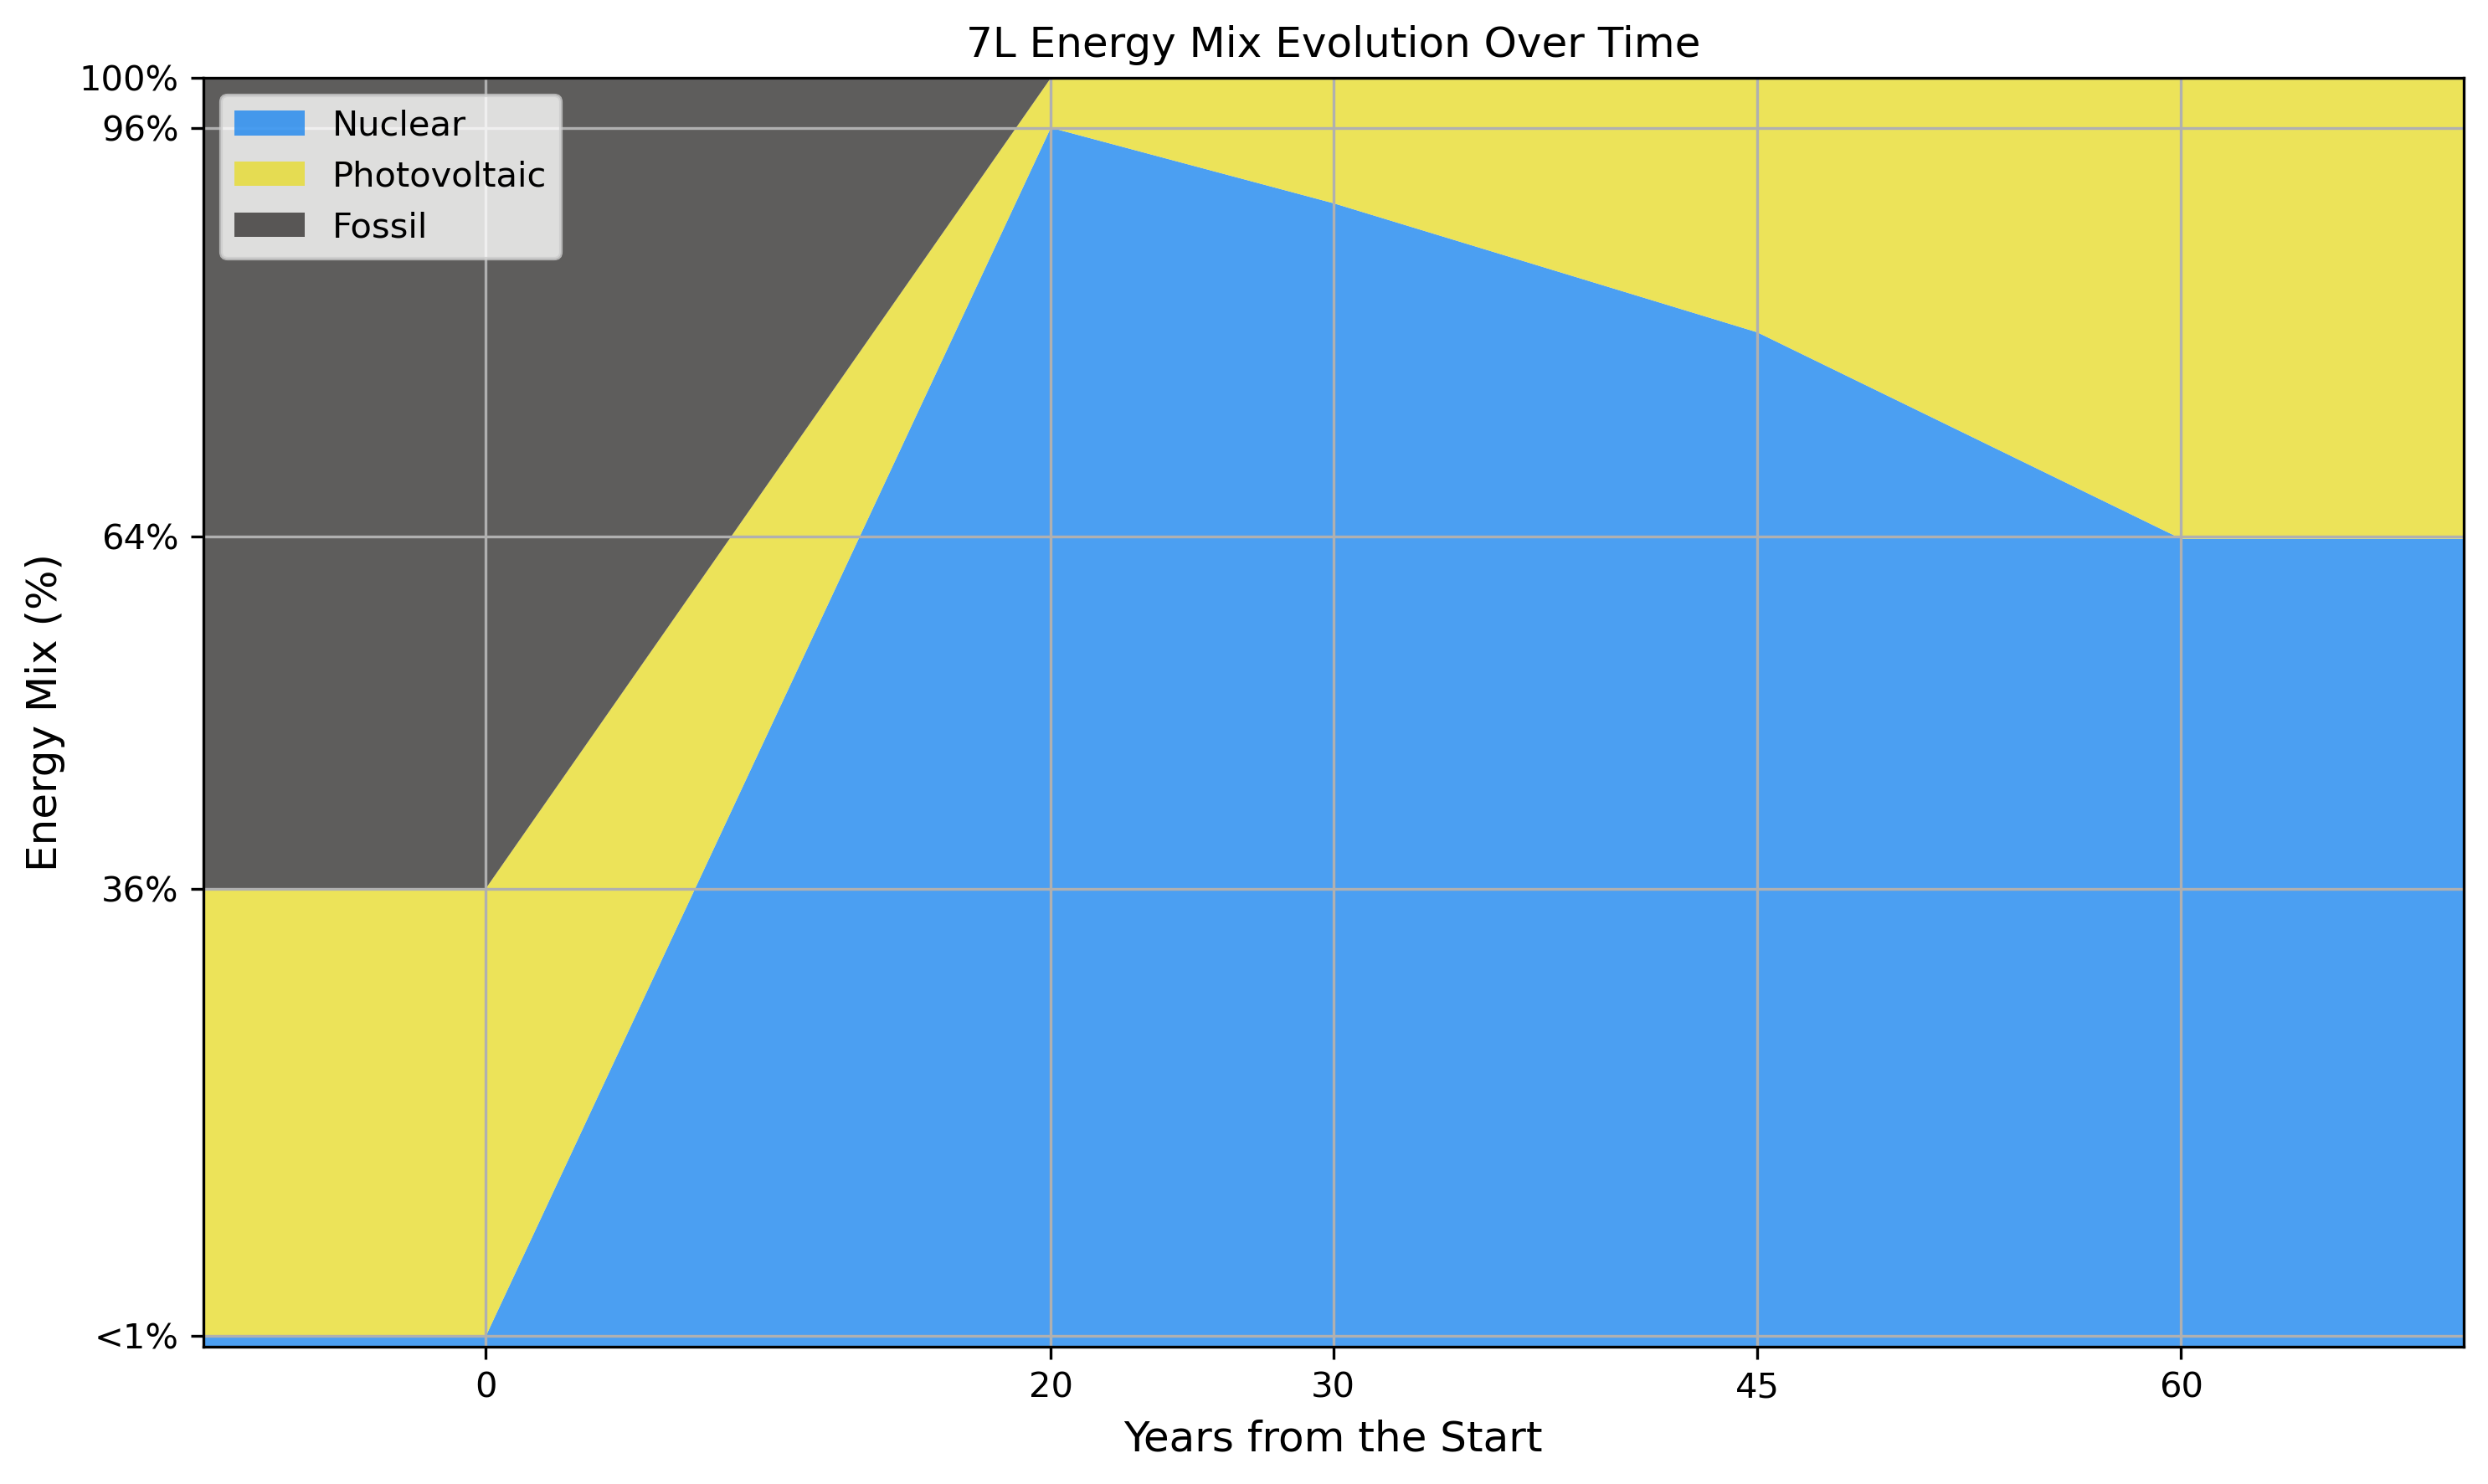
\includegraphics[width=0.8\textwidth]{figures/5_Energy_mix_evolution.png}
    \caption{Local energy mix evolution over time.}
    \label{fig:energy_mix_evolution}
\end{figure}

\paragraph{Residual Fossil Fuel Consumption}
The GHG emissions intensity associated with the residual fossil fuel demand for residential heating are estimated using the processed data, alongside the amount of syngas exported to the market.

The $gCO_{2}eq/kWh$ intensity for this sector is calculated by weighting:
\begin{table}[H]
    \centering
    \begin{tabular}{lc}
        \toprule
        \textbf{Fuel Type} & \textbf{GHG Intensity (gCO$_2$eq/kWh)} \\
        \midrule
        Syngas      & 72.76 \\
        Natural Gas & 550 \\
        \bottomrule
    \end{tabular}
    \caption{GHG intensities for syngas and natural gas in the residential heating sector.}
    \label{tab:residential_heating_ghg}
\end{table}

This impact is zero in the first 20 years of operation, as the plant only provides electricity. From year 21, the introduction of syngas production leads to a growing influence on this sector.

Fossil fuel demand is projected to decrease over time due to improved building energy performance and increased photovoltaic (PV) penetration, while syngas production remains constant — resulting in a gradually increasing contribution to GHG mitigation.


\paragraph{Transportation Sector}
Transport energy consumption data for the region were estimated by scaling national data \cite{eurostat_sankey_2023} according to the population share of the Seven Lakes Region with respect to the national total \cite{istat2023}.

GHG intensities for diesel and gasoline (currently dominant in ground transport) were sourced from \cite{quaschning_co2spec_2025}:
\begin{table}[H]
    \centering
    \begin{tabular}{lcc}
        \toprule
        \textbf{Fuel Type} & \textbf{GHG Intensity (gCO$_2$eq/kWh)} \\
        \midrule
        Diesel    & 266.5 \\
        Gasoline  & 263 \\
        \bottomrule
    \end{tabular}
    \caption{GHG intensities for diesel and gasoline.}
    \label{tab:transportation_ghg}
\end{table}

The impact of the hydrogen produced by the plant is assessed by assuming that it is sold directly to the transportation sector. The resulting GHG intensity is calculated based on the share of energy demand met by:

\begin{table}[H]
    \centering
    \begin{tabular}{lcc}
        \toprule
        \textbf{Energy Carrier} & \textbf{GHG Intensity (gCO$_2$eq/kWh)} \\
        \midrule
        Hydrogen      & 19.39 \\
        Fossil fuels (avg. diesel/gasoline) & 264.75 \\
        \bottomrule
    \end{tabular}
    \caption{GHG intensities for hydrogen and fossil fuels in the transportation sector.}
    \label{tab:transportation_h2_fossil}
\end{table}

Beyond the GHG reduction, it is worth highlighting that hydrogen substitution would also positively affect local air quality due to the elimination of particulate matter emissions typically associated with diesel and gasoline combustion. However, this benefit is not quantified within this study.

\subsubsection{Results}
All results are summarized in the following plots, which illustrate the evolution of GHG emission intensities over time, along with changes in electricity and fossil fuel demand.

\begin{figure}[H]
    \centering
    \begin{minipage}{0.6\textwidth}
        \centering
        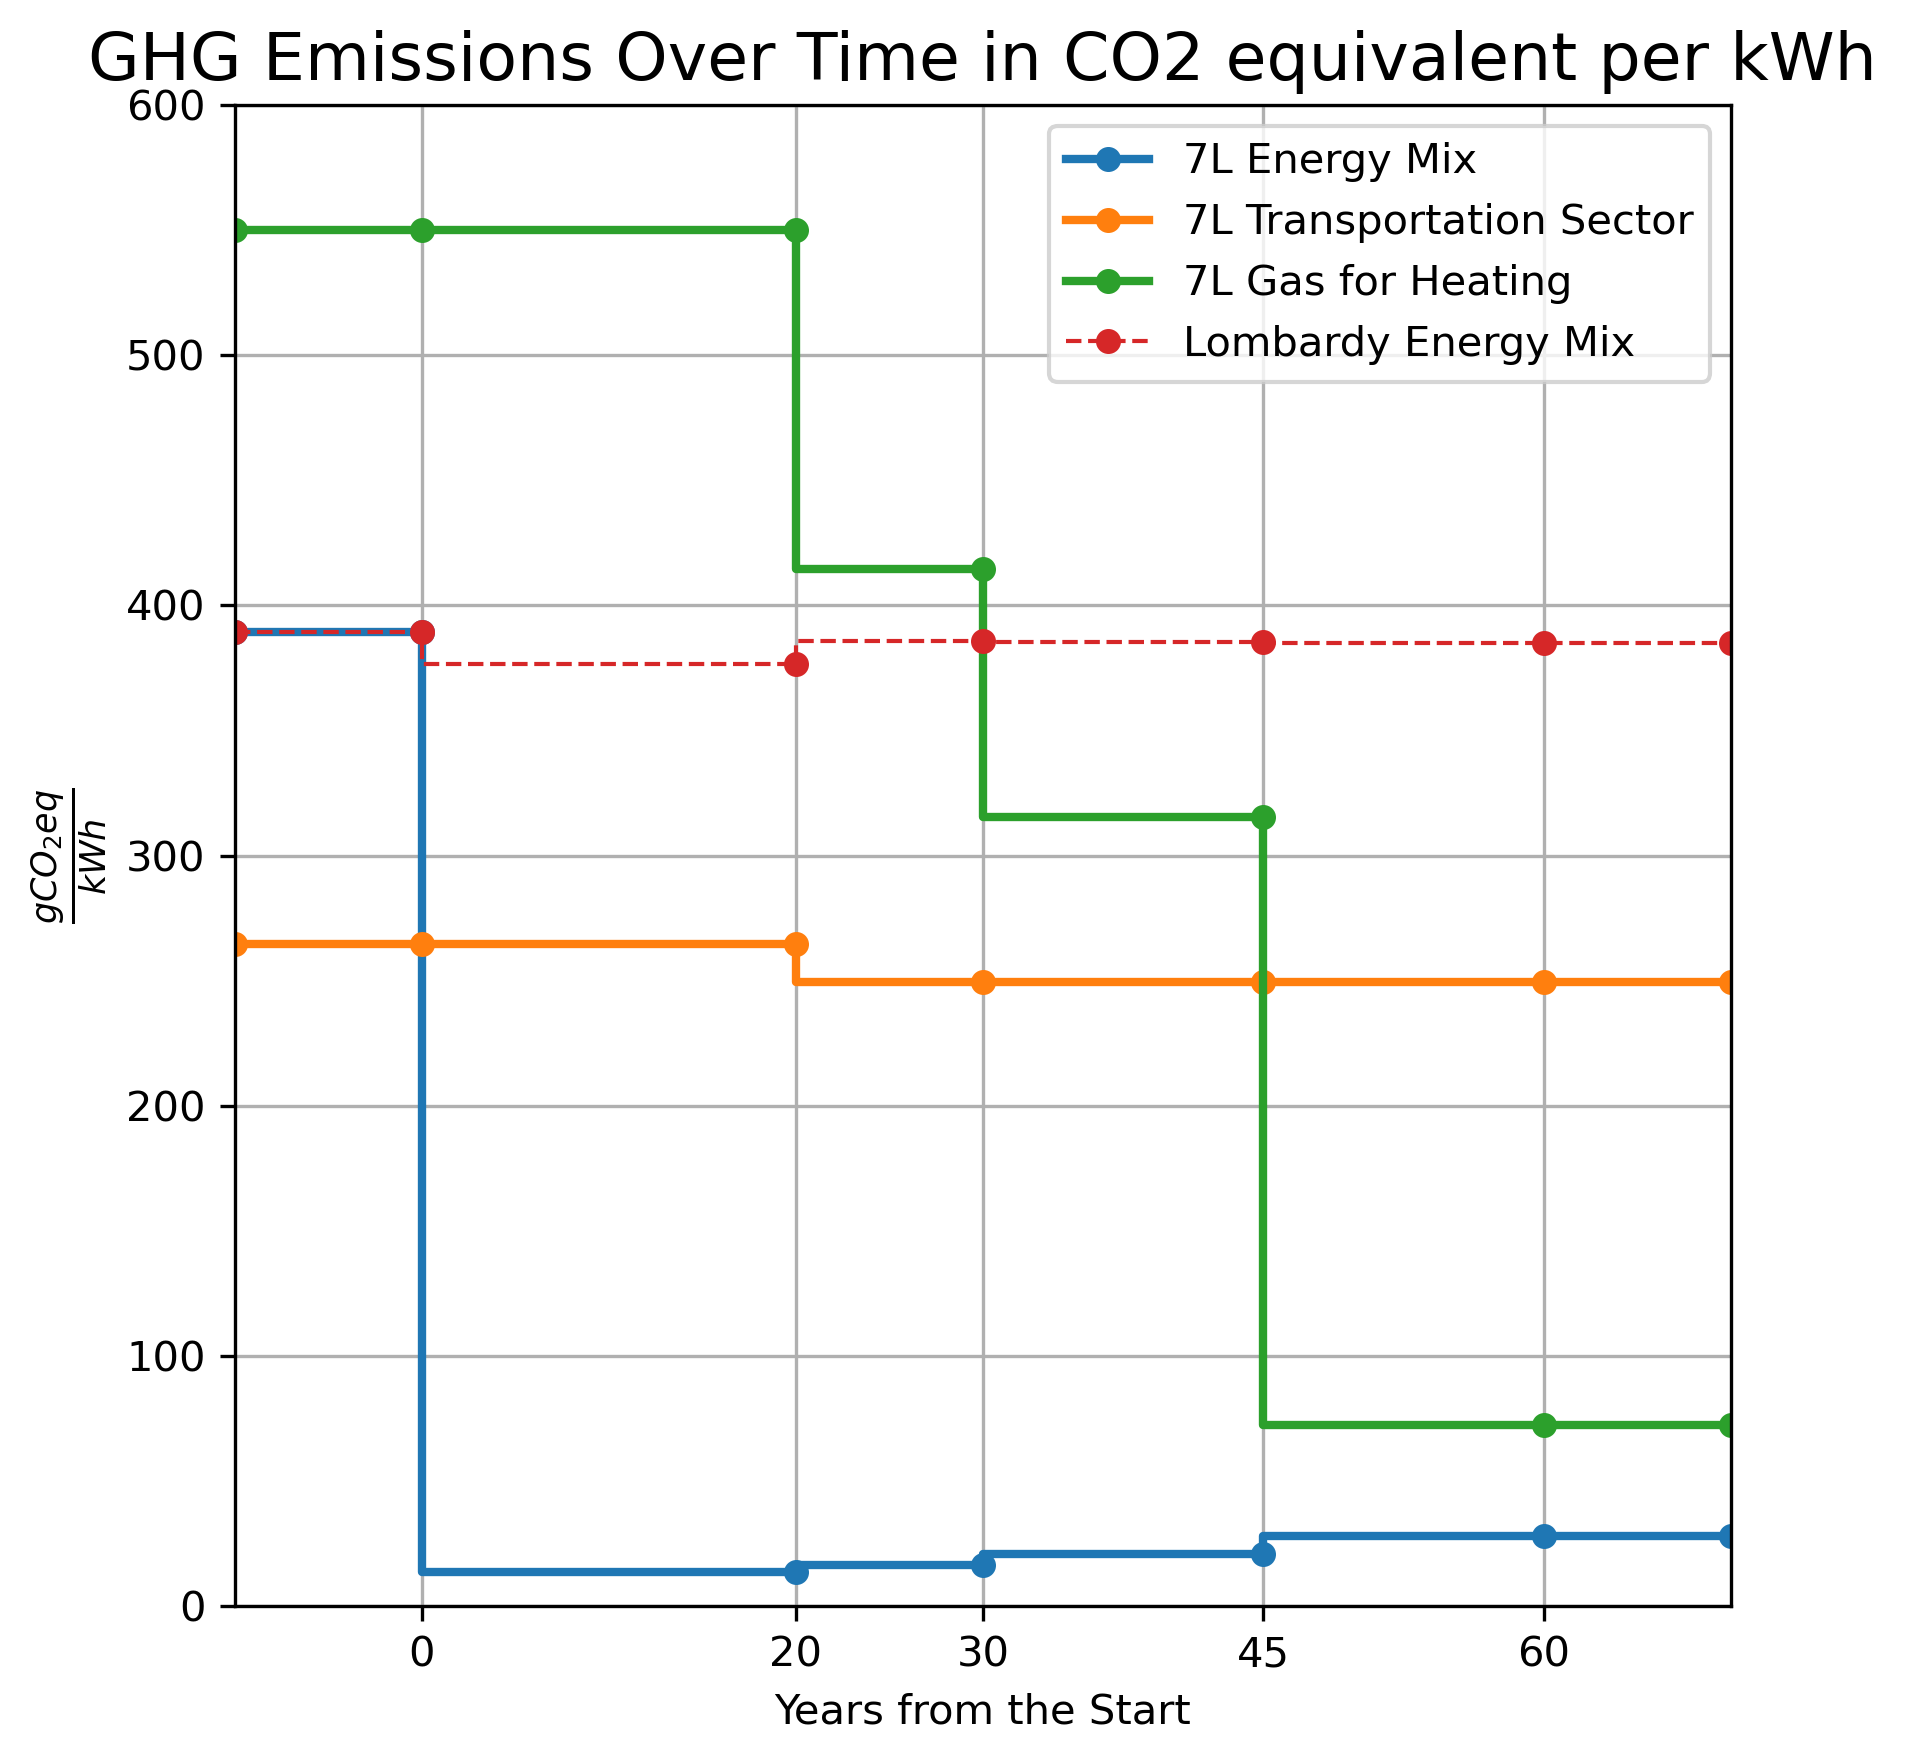
\includegraphics[width=\textwidth]{figures/5_GHG_emissions_over_time.png}
        \caption{GHG emissions intensity over time.}
        \label{fig:ghg_emissions}
    \end{minipage}\hfill
    \begin{minipage}{0.6\textwidth}
        \centering
        
\includegraphics[width=\textwidth]{figures/placeholder.png}
        \caption{Local Net Electricity and Fossil Demand evolution over time.}
        \label{fig:net_electricity_demand}
    \end{minipage}
\end{figure}

The plots highlight several significant trends, including:
\begin{itemize}
    \item ...
    \item ...
    \item ...
\end{itemize}


\subsubsection{Water Usage}
The impact on water resources, primarily required for reactor and Balance of Plant (BoP) operation as well as for the High Temperature Steam Electrolyzer (HTSE) units, is deemed negligible. This is due to the plant's location near Lake Maggiore—one of Italy's largest lakes—which ensures a stable water supply without significant disruption to the basin's hydrological balance or ecosystem.

\subsubsection{Land Use}
One of the key advantages of the proposed project is its minimal land use impact. The compact scale of the facility, combined with its placement in an area already approved for nuclear activities, ensures efficient use of space. The site is located within the Joint Research Centre (JRC) complex, which already hosts research reactors (ESSOR and Ispra-1) and associated nuclear infrastructure. Notably, a containment building is available on-site and is deemed suitable to house at least one of the two planned Small Modular Reactors (SMRs), greatly reducing the need for new construction and environmental disturbance.

\section{Possible Improvements}
\subsection{On the Data Collection}
If the data for each class were obtained from a set of real buildings in the region instead of just one, it would yield better results. Ideally, a statistically significant set of buildings and variable utilization profile could be used. Moreover, it would be beneficial to weigh the simulation data on the real energy requirements of those buildings. This is a much more complex task since it would require extensive data acquisition throughout the year.

From the simulation, humidification and dehumidification electricity needs are neglected since these plants are rarely installed today. A better evaluation would consider the possible future share of air treatment plants in the residential sector. For the purpose of this study, the share of installed air conditioning systems for cooling was assumed constant throughout the years, but it might increase in the future.

\subsubsection{Renewable Energy Sources}
Solar-thermal systems were neglected since they are considered not very impactful and complex to evaluate.

\subsubsection{Conversion to Primary Energy}
Time-dependent efficiency for heat pumps, taking into account the ambient temperature could improve the model.

\subsubsection{Other Electricity Demand}
This is the most complex contribution to evaluate, especially considering that it is not easy to forecast how electricity consumption will evolve in 60 years. Collecting a statistically significant number of data from the region regarding the type of appliances installed and their consumption would improve the simulation.
For the purpose of this study the appliances demand was assumed constant throughout the years.

\subsection{On the Plant Modelling and Simulation}
The Modelica model could be utilized to analyze the dynamic response of the plant to transient conditions, thereby evaluating the system's adequacy and frequency control capabilities. This analysis could focus on critical periods, such as specific days of the year characterized by significant demand oscillations.

Additionally, buffers with limited capacity could be modeled to further understand their impact on system dynamics. The hydrogen plant could be simulated to partially shut down some HTSE units, allowing for better adaptation to demand variations.

Incorporating chemical kinetics into the methanation model could enhance the simulation of the plant's dynamic response to transient conditions. Furthermore, the optimization of hydrogen tapped for market consumption could be based on a detailed analysis of the transportation sector.

Lastly, the sizing of the entire plant should be optimized based on a comprehensive economic assessment.

\subsection{On the Economic Study}

\section{Conclusion}